\chapter{Cronograma}

\begin{figure}[h]
    \centering

    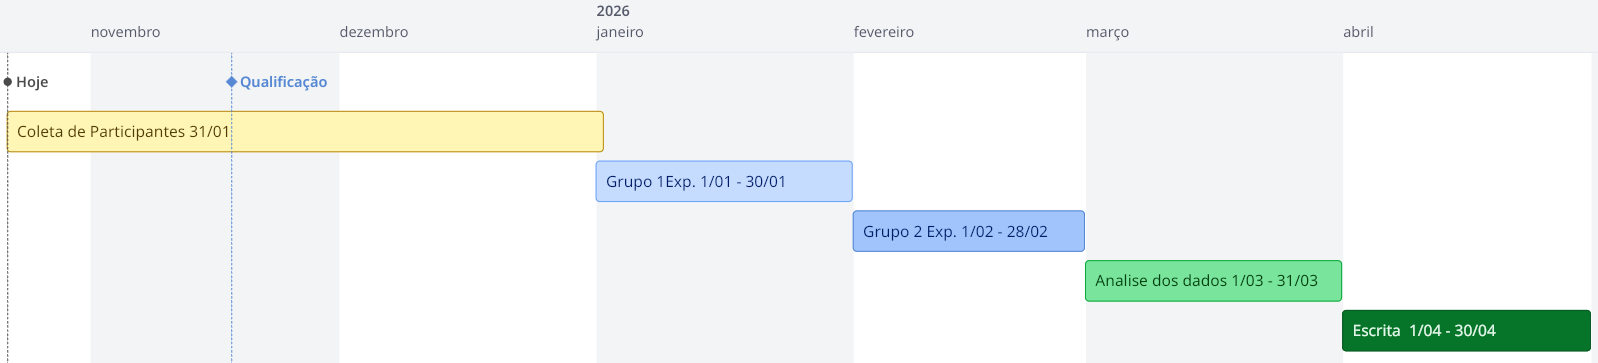
\includegraphics[width=1\textwidth]{imgs/Cronograma.png}
    \caption{Cronograma do trabalho}
    \label{fig:Cronograma}
\end{figure}

O cronograma dessa qualificação foi organizado de forma a contemplar todas as etapas do projeto, desde a coleta dos participantes até a escrita final da dissertação.

A coleta de participantes teve início em agosto de 2025 e se estenderá até o dia 31 de dezembro de 2025. Durante esse período, o recrutamento será feito por meio de questionários online compartilhados em fóruns, redes sociais e servidores da comunidade do jogo Among’Us na plataforma Discord. Essa fase visa reunir uma amostra diversificada, incluindo tanto jogadores habituais quanto não jogadores, e, se possível, pessoas diagnosticadas com TDAH.

A primeira fase de experimentação ocorrerá entre os dias 1º de janeiro e 31 de janeiro de 2026, com o Grupo 1. Durante essa etapa, os participantes serão divididos em subgrupos com base em sua familiaridade com jogos multiplayer (jogadores, não jogadores e grupos mistos) e participarão de sessões semanais dos jogos Among’Us e Overcooked. Serão realizadas coletas regulares de dados por meio de questionários e observações das interações durante as jogatinas.

A segunda fase de experimentação, com o Grupo 2, acontecerá entre 1º de fevereiro de 2026 e 28 de fevereiro de 2026, seguindo a mesma lógica da fase anterior, mas com novos participantes e diferentes composições.

O mês de março de 2026 será dedicado à análise dos dados coletados ao longo dos experimentos. Serão comparadas as respostas dos questionários de habilidades sociais, observações comportamentais e, possivelmente, registros de áudio dos participantes, com o objetivo de identificar padrões de desenvolvimento ou uso de habilidades sociais.

Por fim, o mês de abril de 2026 será reservado para a redação e finalização da dissertação, integrando os resultados obtidos com a fundamentação teórica e a discussão crítica sobre os achados da pesquisa.
